\documentclass[conference]{IEEEtran}
\IEEEoverridecommandlockouts
\usepackage{cite}
\usepackage{amsmath,amssymb,amsfonts}
\usepackage[linesnumbered,ruled]{algorithm2e}
\usepackage{graphicx}
\usepackage{textcomp}
\usepackage{xcolor}
\usepackage{listings}
 \usepackage{algpseudocode}
\usepackage{xfp}
\usepackage{float}
\usepackage{algorithm}
\usepackage[section]{placeins}
\begin{document}
	
	\section*{Methodology}
	
	The proposed scheme consists of several sub modules as
	shown in the flow diagram in Fig.\ref{fig:k1}. All the modules of the
	proposed scheme have been written in Python 3.9.
	
	The code is provided here: https://github.com/CaffineAddic/ Wavelet\_transforms\_in\_schlieren\_flame\_images
	
	\begin{figure}[H]
		\centering
		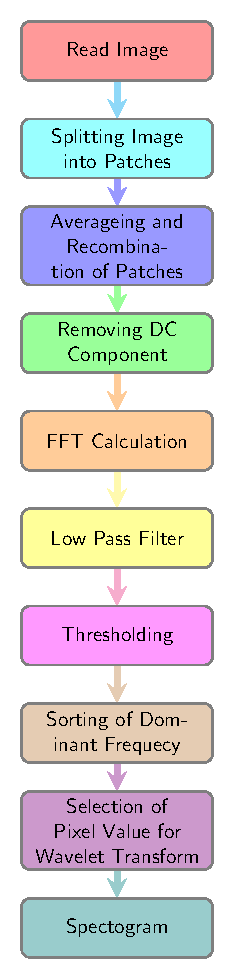
\includegraphics[scale=1.11]{plot/meth.pdf}
		\caption{Flowchart of the image processing procedure}\label{fig:k1}
			\end{figure}
			An exemplary instantaneous Schlieren image of the
			liquid spray from the high-speed image sequence is shown
			in Fig. \ref{fig:k2} 
	
	\begin{algorithm}
		\caption{FFT Analysis and Visualization}
		\begin{algorithmic}[1]
			\State \textbf{Input:} $\{P_{i}\}_{i=1}^{N}$, a set of $N$ input data points\State \textbf{Output:} $\{F_{i}\}_{i=1}^{M}$, a set of $M$ output frequency distributions\Procedure{DataPreprocessing}{}\State Load input data: $\{P_{i}\}_{i=1}^{N}$\State Select time range: $T = [t_{start}, t_{end}]$\State Crop data: $D = \{P_{i}\}_{i=1}^{N} \cap T$\EndProcedure\Procedure{Patchification}{}\State Create patches: $Patches = \{P_{i}\}_{i=1}^{N} \mapsto \{Patches_{i}\}_{i=1}^{N}$\State Calculate mean of patches: $\{Mean_{i}\}_{i=1}^{N}$\EndProcedure\Procedure{FFT}{}\State Calculate FFT of mean: $\{FFT_{i}\}_{i=1}^{N}$\State Filter FFT: $\{Filtered_{i}\}_{i=1}^{N}$\EndProcedure\Procedure{FrequencyDistribution}{}\State Calculate frequency distribution: $\{F_{i}\}_{i=1}^{M}$\State Sort and arrange data: $\{F_{i}\}_{i=1}^{M} \mapsto \{Sorted_{i}\}_{i=1}^{M}$\EndProcedure\Procedure{Visualization}{}\State Plot frequency distribution: $\{Sorted_{i}\}_{i=1}^{M} \mapsto \{Plot_{i}\}_{i=1}^{M}$\State Save plots: $\{Plot_{i}\}_{i=1}^{M} \mapsto \{File_{i}\}_{i=1}^{M}$\EndProcedure
		\end{algorithmic}
	\end{algorithm}
	
	\begin{figure}[H]
	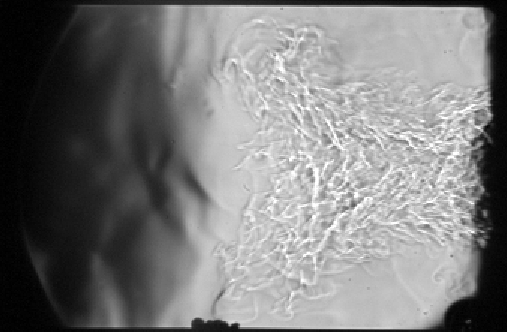
\includegraphics[scale=.51]{plot/flame.png}
	\caption{Image obtained from Schlieren imaging}\label{fig:k2}
\end{figure}	


	
	\subsection{Patches Splitting and Recombination after Averaging}
	The Schlieren images are high resolution to reduce computational overhead and time, the images are split into small image patches, further in each patch the average value of the entire patch is calculated and integrated together to form pooled images with a lower resolution while preserving information.
	
A sample image after the process is depicted in Fig. \ref{fig:k3}. Here, the image has been color-mapped to a specific scheme and is presented with a color bar, allowing for a visual representation of pixel intensity.
	
		\begin{figure}[H]
		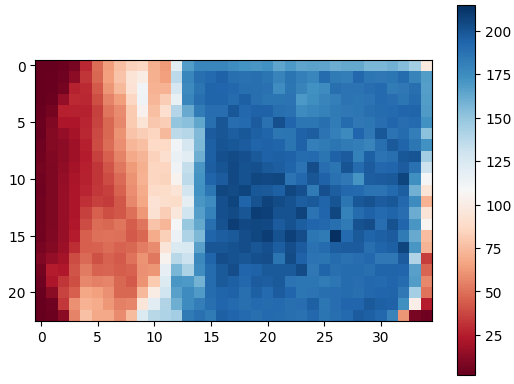
\includegraphics[scale=.51]{plot/pool.png}
		\caption{Image obtained after integrating the average of patches}\label{fig:k3}
	\end{figure}
	
\subsection{DC component removal \& Fast Fourier Transform (FFT) calculation}


For each post-integrated image in the sequence, the average of all pixel values is computed and subtracted from each pixel to eliminate the DC component Fig. \ref{fig:k4}. This process, known as centering the data or mean normalization, helps remove bias in the dataset. After applying mean normalization to all images in the series, the FFT is calculated for each pixel, spanning across the entire integrated image sequence.

		\begin{figure}[H]
	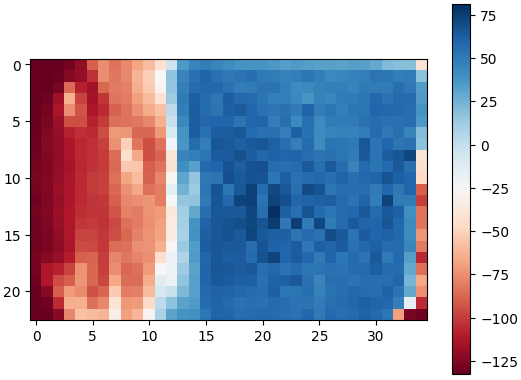
\includegraphics[scale=.51]{plot/pool2.png}
	\caption{Image after mean normalization}\label{fig:k4}
\end{figure}

\subsection{Low Pass Filtering (LPF)\& Thresholding}

LPT filtering is utilized on the FFT series to eliminate noise, particularly targeting the low-frequency components. Additionally, a thresholding process based on the FFT amplitude is implemented to filter out frequency components with low amplitudes. This dual approach helps to enhance the quality of the FFT data by reducing noise and focusing on significant frequency components.

\subsection{Sorting of Dominant Frequencies}

The frequency values in the FFT array are sorted according to their FFT amplitudes. Subsequently, the highest amplitude value from each sorted FFT array is integrated into an image to visualize the most dominant frequency for each pixel. This process allows for the observation of the primary frequency components across the image, as illustrated in Fig. \ref{fig:k5}. Further the FFT amplitude of each dominating frequency is shown in Fig. \ref{fig:k6}.

		\begin{figure}[H]
	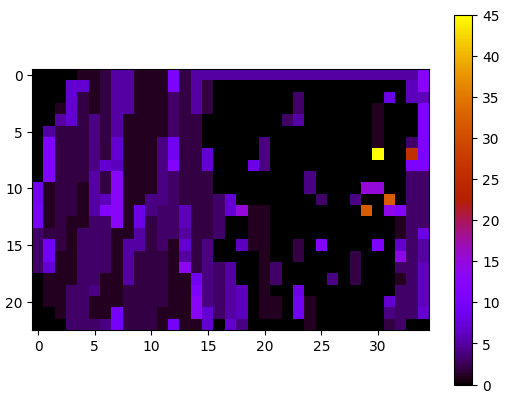
\includegraphics[scale=.51]{plot/freq.png}
	\caption{Image displaying all the dominant frequency for each pixel}\label{fig:k5}
\end{figure}

		\begin{figure}[H]
	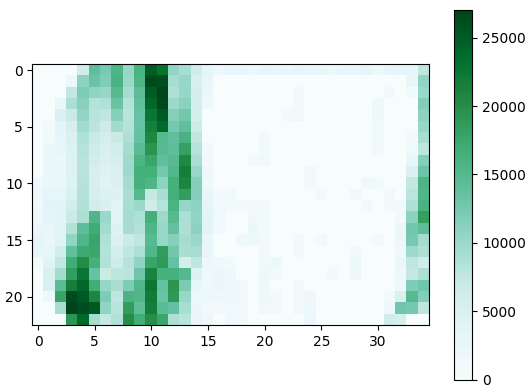
\includegraphics[scale=.51]{plot/ampli.png}
	\caption{Corresponding amplitude for each frequency in Fig. \ref{fig:k5}}\label{fig:k6}
\end{figure}

\subsection{Wavelet Transform Calculation and Spectrogram}

From the dominant frequency flame image, a specific pixel of interest is chosen to extract temporal information of the frequencies present. This involves identifying the time duration and the frequencies displayed by the selected pixel. This targeted approach allows for a detailed analysis of the temporal characteristics and frequency components exhibited by the pixel under investigation. Further spectrogram is plotted to display that information as in Fig. \ref{fig:k7}.

\begin{algorithm}
	\caption{Wavelet Analysis of Pixel-Selected Intensity Time Series}
	\begin{algorithmic}[1]
		\State Input: $pl$ (Pixel location) [User Input]\State $s = data[:, pl[0], pl[1]]$\State $t = gen\_time(data.shape[0])$\State $t = t/fs + init\_time$\State $sc = gen\_scale(min\_scale, max\_scale)$\State $c, f = wt(s, sc, wavelet, fs)$\State Plot scalogram using $t$, $f$, and $c$ with 'inferno' colormap\State Save to file 'calo-' + $pl$ + '.png'
\end{algorithmic}
\end{algorithm}

		\begin{figure}[H]
	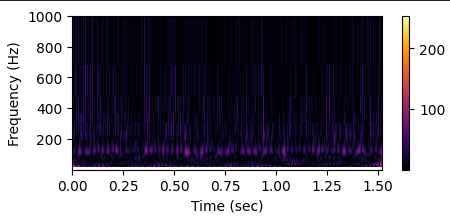
\includegraphics[scale=.51]{plot/spect.png}
	\caption{The spectrogram of the pixel of interest.}\label{fig:k7}
\end{figure}


\end{document}
